% % % %
% % % % Overview
% % % %
\section{Overview} 

\subsection{Competition Details}
\begin{frame}\frametitle{Data} 
\par \textbf{Goal}: Identify signs of diabetic retinopathy in eye images
\par \textbf{Given}: 35126 images for training, 53576 images in test set
\par Images are big: 2500x2000 and larger
\par Compressed data size: 88Gb

\vspace{5pt}

\begin{tabular}{|@{}c@{}|@{}c@{}|@{}c@{}|@{}c@{}|@{}c@{}|}
\hline
	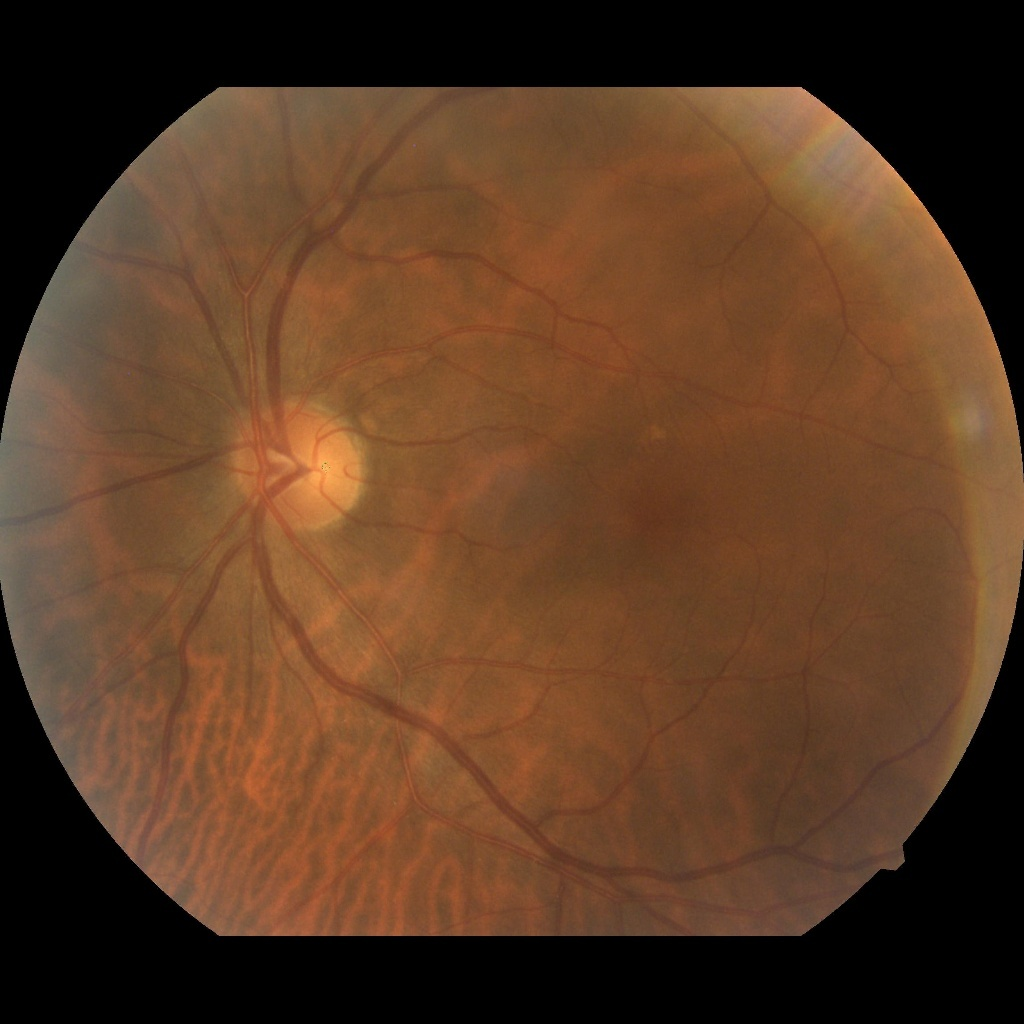
\includegraphics[width=0.2\textwidth]{pics/classified_samples/197_left_0.jpg} &
	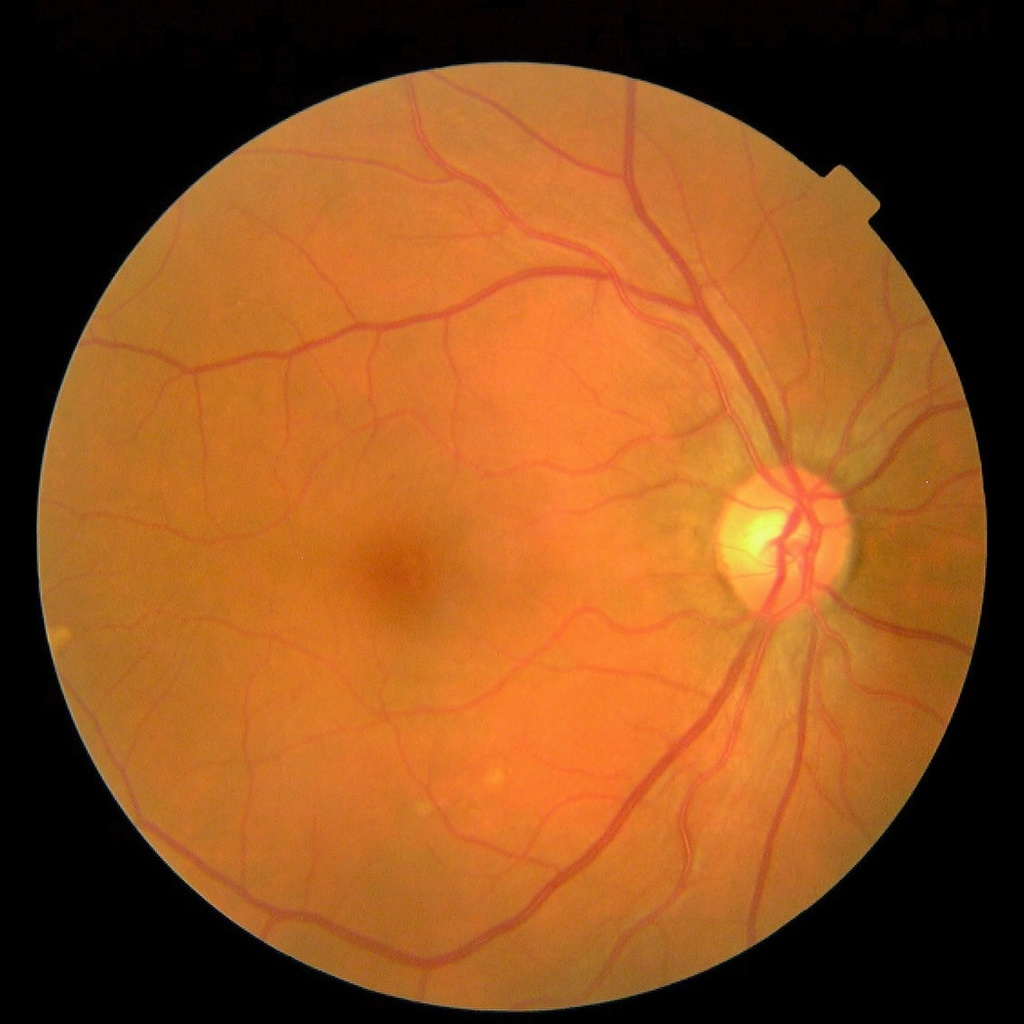
\includegraphics[width=0.2\textwidth]{pics/classified_samples/204_right_1.jpg} &
	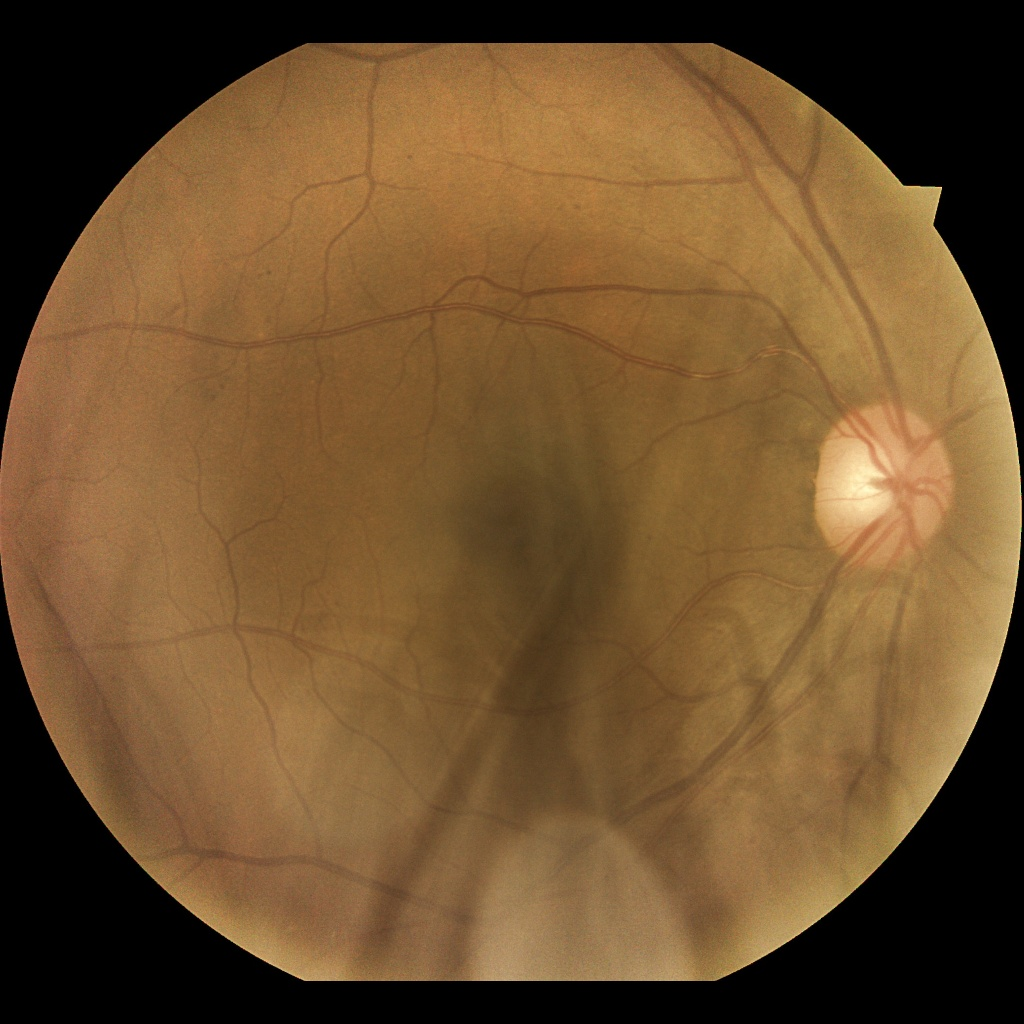
\includegraphics[width=0.2\textwidth]{pics/classified_samples/82_right_2.jpg} &
	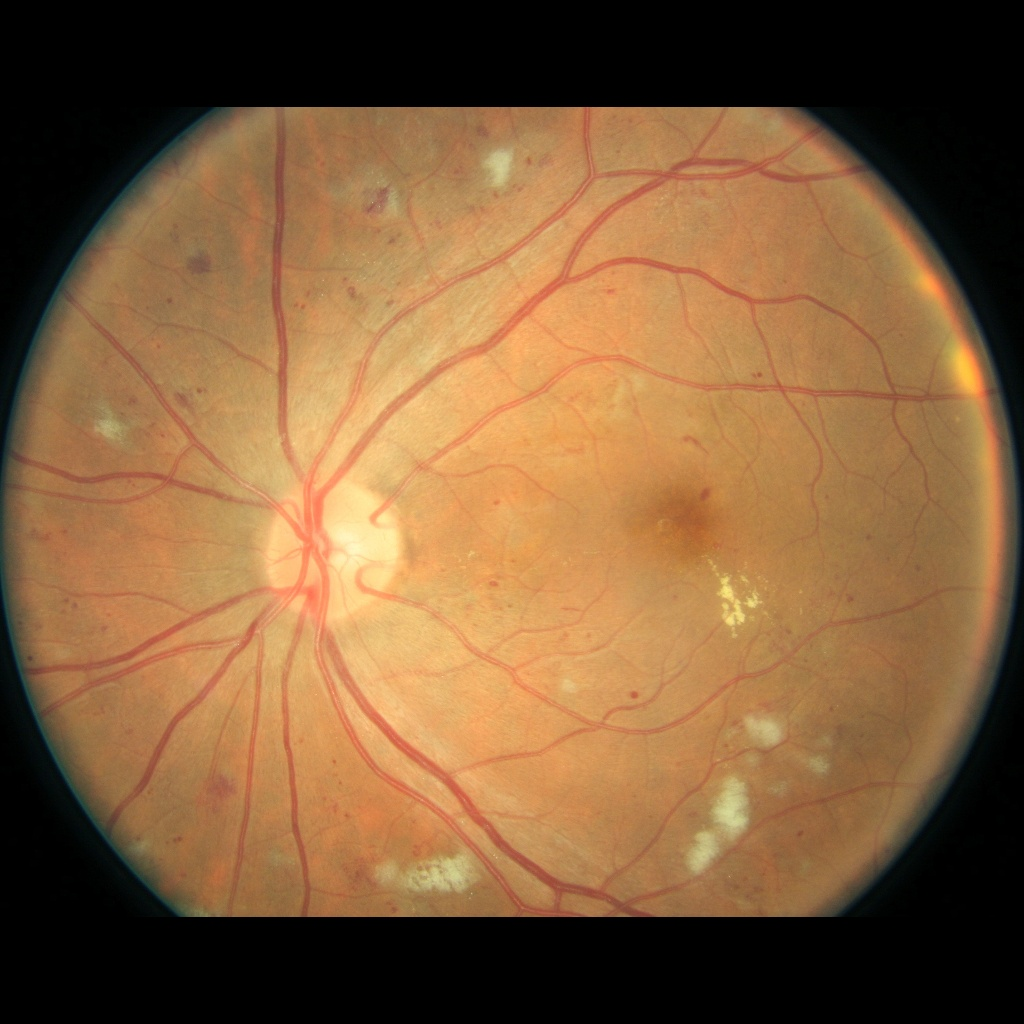
\includegraphics[width=0.2\textwidth]{pics/classified_samples/687_right_3.jpg} &
	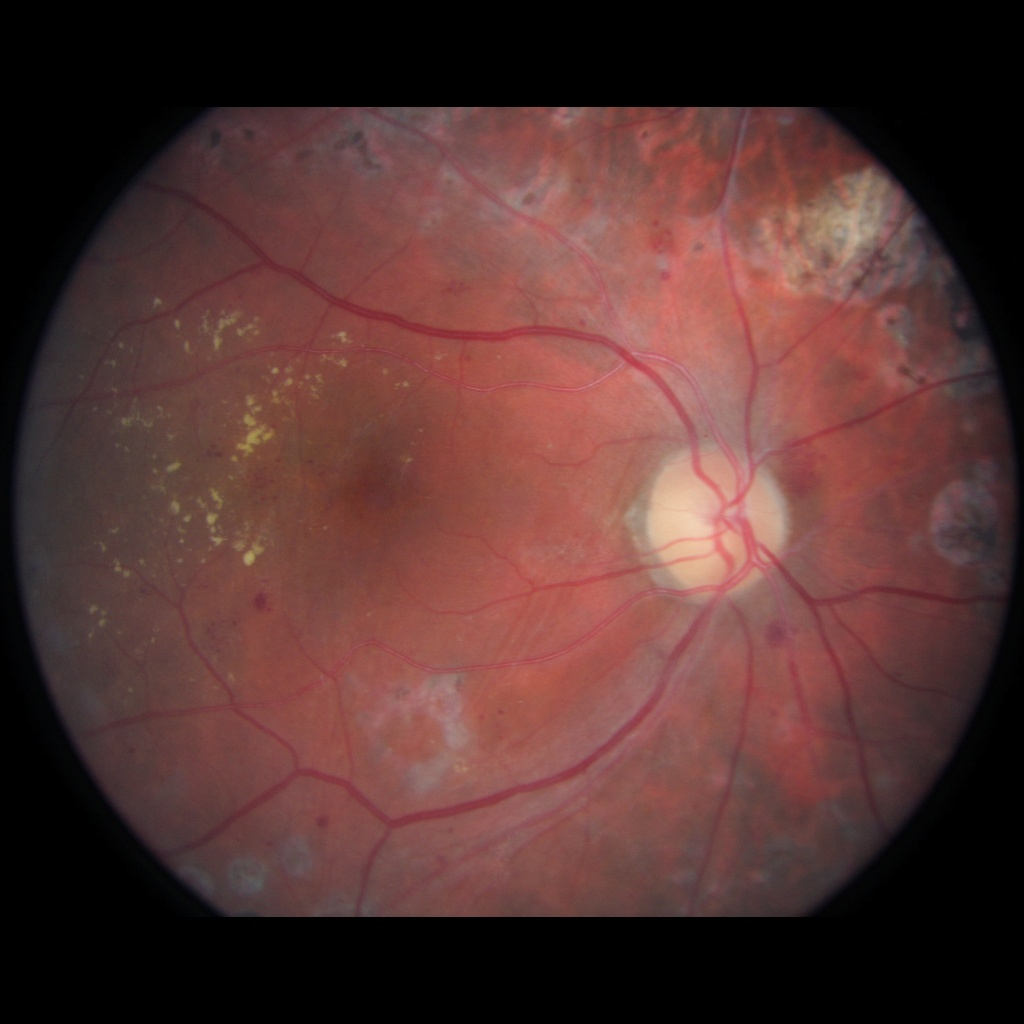
\includegraphics[width=0.2\textwidth]{pics/classified_samples/2496_left_4.jpg} \\\noalign{\vspace{-0.15cm}}
\hline

Normal & Mild & Moderate & Severe & Proliferative \\

\hline
 \specialcell{25810\\ \footnotesize{73.48\%}}  & 
 \specialcell{2443\\\footnotesize6.96\%} & 
 \specialcell{5292\\\footnotesize15.07\%} & 
 \specialcell{873\\\footnotesize2.48\%} & 
 \specialcell{708\\\footnotesize2.01\%} \\

\hline
\end{tabular}

\end{frame}

\begin{frame}\frametitle{Quality metric I: Cohen's kappa}
%\footnotesize
Cohen's kappa measures the agreement between two raters A and B who each classify $N$ items into $C$ mutually exclusive categories. 

\[ \kappa = \frac{p_o - p_e}{1 - p_e} = 1- \frac{1 - p_o}{1 - p_e}, \]

where
\begin{itemize}
\item $p_o$ is the relative observed agreement among raters
\item $p_e$ is the hypothetical probability of chance agreement
\end{itemize}

\par \[\kappa=\frac{Pr[A=B]-Pr[A=B|A \text{ and }B \text{ independent}]}{1-Pr[A=B|A \text{ and }B \text{ independent}]} \]

\par If the raters are in complete agreement then $\kappa = 1$. 
\end{frame}

\begin{frame}\frametitle{Quality metric I: Cohen's kappa (simple example)}
\footnotesize
\begin{table}[]
\centering
\begin{tabular}{c|c|c|c|c|c}
\cline{3-5}
\multicolumn{2}{c|}{\multirow{2}{*}{}}           & \multicolumn{3}{c|}{A} &                            \\ \cline{3-6} 
\multicolumn{2}{c|}{}                            & 1      & 2     & 3     & \multicolumn{1}{c|}{Total} \\ \hline
\multicolumn{1}{|c|}{\multirow{3}{*}{B}} & 1     & 55     & 5     & 5     & \multicolumn{1}{c|}{65}    \\ \cline{2-6} 
\multicolumn{1}{|c|}{}                   & 2     & 15     & 45    & 15    & \multicolumn{1}{c|}{75}    \\ \cline{2-6} 
\multicolumn{1}{|c|}{}                   & 3     & 5      & 10    & 45    & \multicolumn{1}{c|}{60}    \\ \hline
                                         & Total & 75     & 60    & 65    & \multicolumn{1}{c|}{200}   \\ \cline{2-6} 
\end{tabular}
\end{table}

\par \[ p_o = P(1)+P(2)+P(3) = 0.725 \]
\par \[ p_e = P(1|A)P(1|B)+P(2|A)P(2|B)+P(3|A)P(3|B) = 0.313 \]
\par \[ \kappa = \frac{p_o - p_e}{1 - p_e} = 0.588 \]

\end{frame}

\begin{frame}\frametitle{Quality metric II: quadratic weighted kappa} 
\small
\vspace{-15pt}

\footnotesize { % TODO: rewrite
Images have five possible ratings, 0,1,2,3,4.  Image is characterized by a tuple $(e_a,e_b)$, which corresponds to scores by $Rater A$ (human) and $Rater B$ (predicted). 

{\bf Quadratic weighted kappa} is calculated as: 
\vspace{-2pt}
\[ \kappa=1-\frac{\sum_{i,j}w_{i,j}O_{i,j}}{\sum_{i,j}w_{i,j}E_{i,j}}, \]
\vspace{-5pt}
where:
\vspace{1pt}
\begin{itemize}
\item $O$ is $N\times N$ histogram matrix, such that $O_{i,j}$ corresponds to the number of images that received a rating $i$ by $A$ and a rating $j$ by $B$. 

\item $E$, is $N\times N$ histogram matrix of expected ratings. $E$ calculated, assuming that there is no correlation between rating scores.  This is calculated as the outer product between each rater's histogram vector of ratings, normalized such that $E$ and $O$ have the same sum.

\item $w$ is $N\times N$ matrix of weights, which calculated based on the difference between raters' scores:
\vspace{-1pt}
\[ w_{i,j} = \frac{\left(i-j\right)^2}{\left(N-1\right)^2} \]

\end{itemize}

}

\end{frame}

\subsection{Competition Results}

\begin{frame}\frametitle{Private leaderboard} 
\vspace{-20pt}
\begin{center}
\begin{figure}
\adjincludegraphics[width=\textwidth,trim={1cm 12cm 1cm 2.5cm},clip]{pics/private_lb_selected.pdf}
\end{figure}
\end{center}
\end{frame}


\begin{frame}\frametitle{Teams distribution on private LB} 
\vspace{-20pt}
\begin{center}
%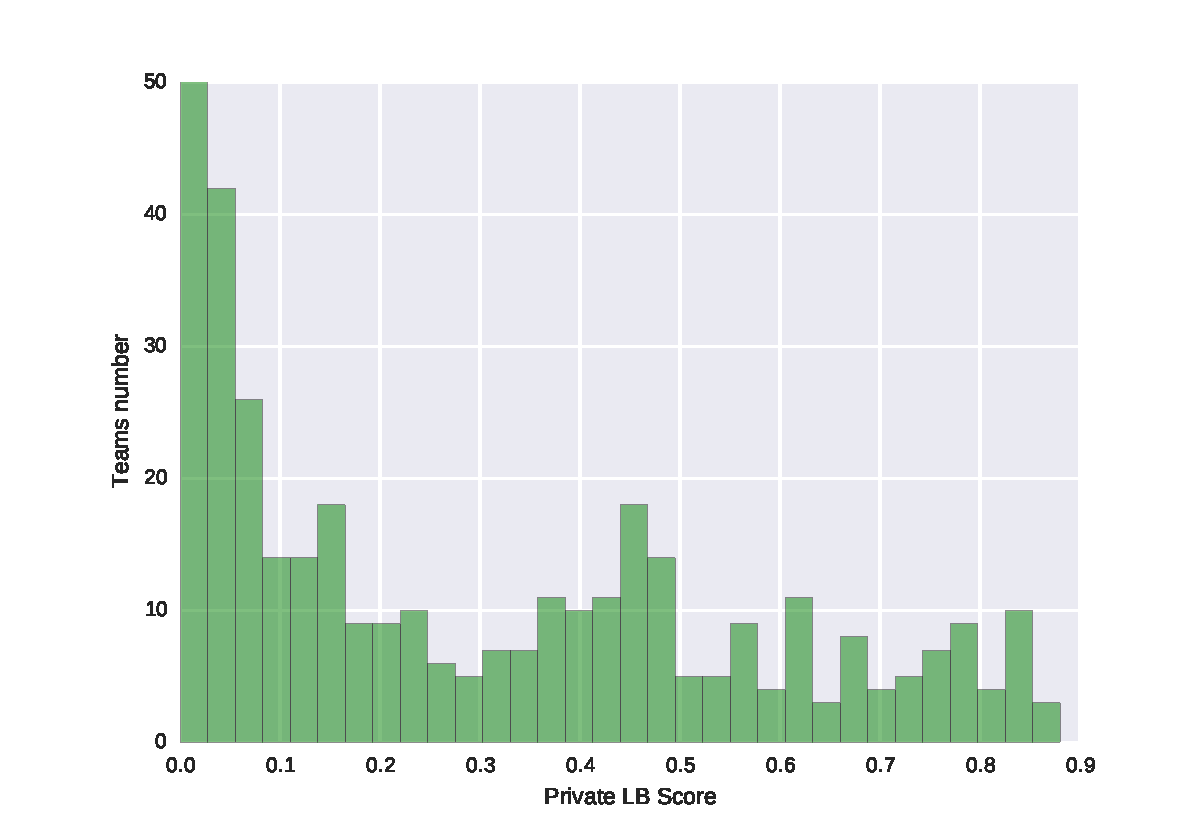
\includegraphics[width=\textwidth]{pics/private_lb_distribution.pdf}
\adjincludegraphics[width=\textwidth,trim={1.5cm 0cm 1.5cm 3cm},clip]{pics/private_lb_distribution.pdf}
\end{center}
\end{frame}


\begin{frame}\frametitle{} 
\begin{center}
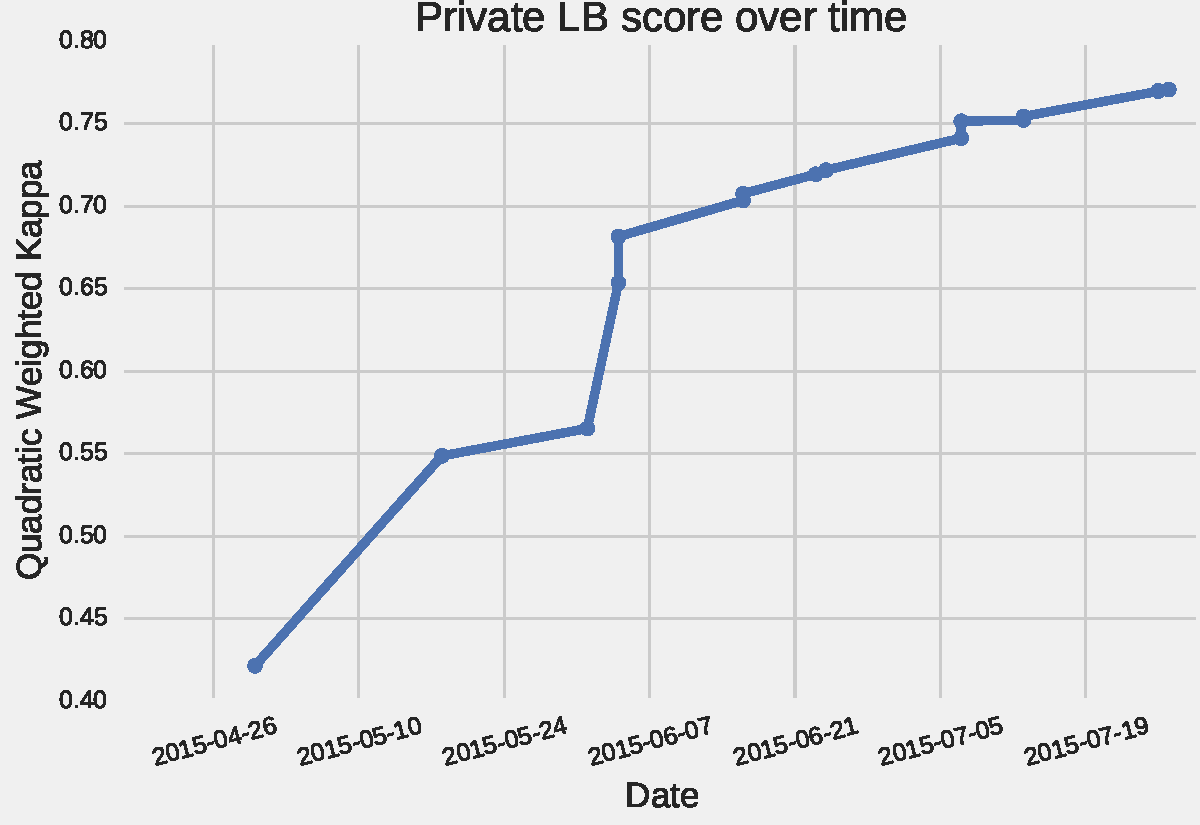
\includegraphics[width=\textwidth]{pics/private_lb_score_increase.pdf}
\end{center}
\end{frame}

%\begin{frame}\frametitle{} 
%\par final leaderboard
%\par + provide leaderboard histogram
%\par + plot score over time
%\end{frame}
